\documentclass{article}
\usepackage[utf8]{inputenc}
\usepackage{amsmath,amssymb}
\usepackage{graphicx}
\usepackage{float}
\usepackage{subcaption}
\usepackage{geometry}
\geometry{
    a4paper,
    total={170mm,257mm},
    left=20mm,
    right=20mm,
    top=20mm,
}
\usepackage{listings} % code listings
\lstset{framextopmargin=0pt,frame=lines}
\lstset{
    language=Matlab,
    basicstyle=\footnotesize\ttfamily,
    breaklines=true,
    tabsize=4,
    keepspaces=true,
    columns=flexible,
    % backgroundcolor=\color[gray]{0.9},
    frame=single,
    breaklines=true,%
    morekeywords={matlab2tikz},
    keywordstyle=\color{blue},%
    morekeywords=[2]{1}, keywordstyle=[2]{\color{black}},
    identifierstyle=\color{black},%
    stringstyle=\color{mylilas},
    commentstyle=\color{mygreen},%
    showstringspaces=false,%without this there will be a symbol in the places where there is a space
    numbers=left,
    numberstyle={\tiny \color{black}},% size of the numbers
    numbersep=9pt, % this defines how far the numbers are from the text
    emph=[1]{for,end,break},emphstyle=[1]\color{red}, %some words to emphasise
    %emph=[2]{word1,word2}, emphstyle=[2]{style},
}
\usepackage{color} %red, green, blue, yellow, cyan, magenta, black, white
\definecolor{mygreen}{RGB}{28,172,0} % color values Red, Green, Blue
\definecolor{mylilas}{RGB}{170,55,241}

\title{ENV-541 Sensor Orientation\\Lab 1 - Stochastic Processes}
\author{Michael Spieler}
\date{October 5, 2018}

\begin{document}

\maketitle

\section*{1 Noise realizations plot}

\begin{figure}[H]
\centering
\begin{subfigure}[t]{0.49\textwidth}
\centering
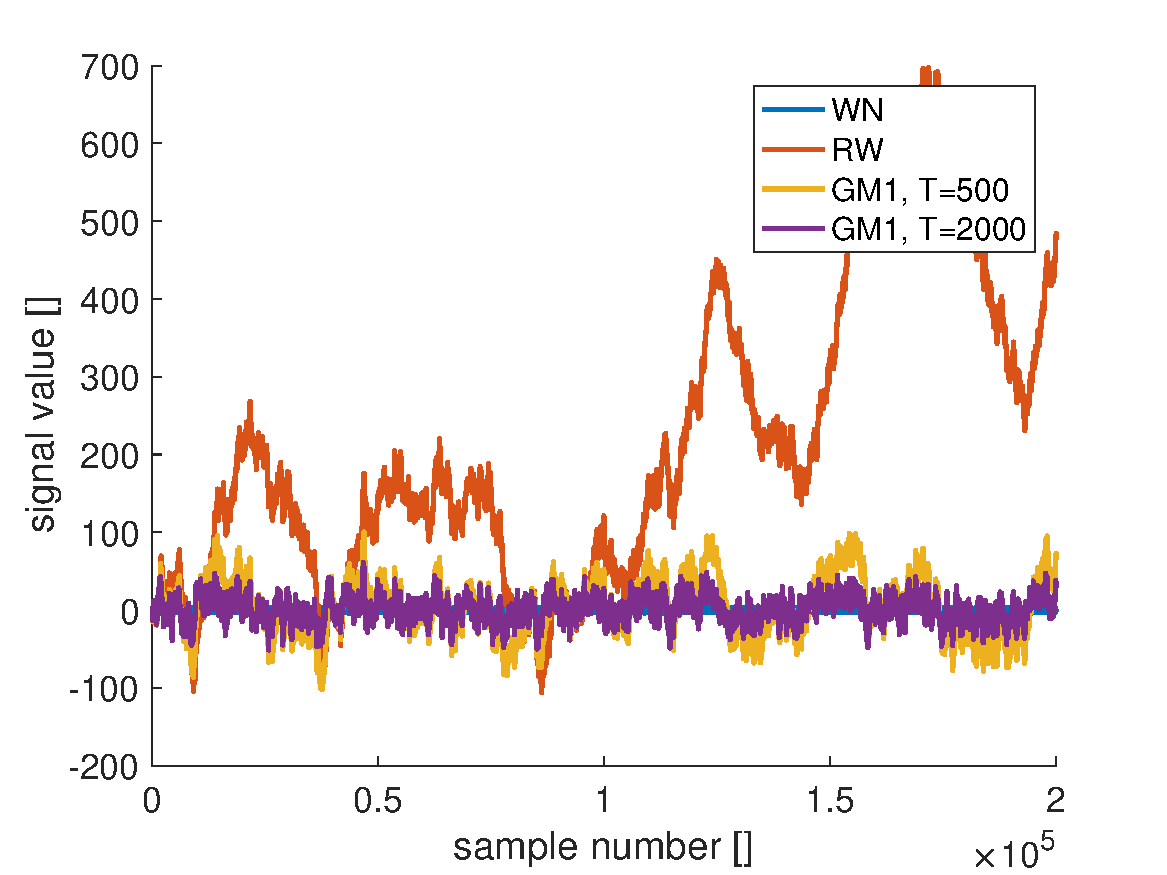
\includegraphics[width=\textwidth]{signal1}
\end{subfigure}
~
\begin{subfigure}[t]{0.49\textwidth}
\centering
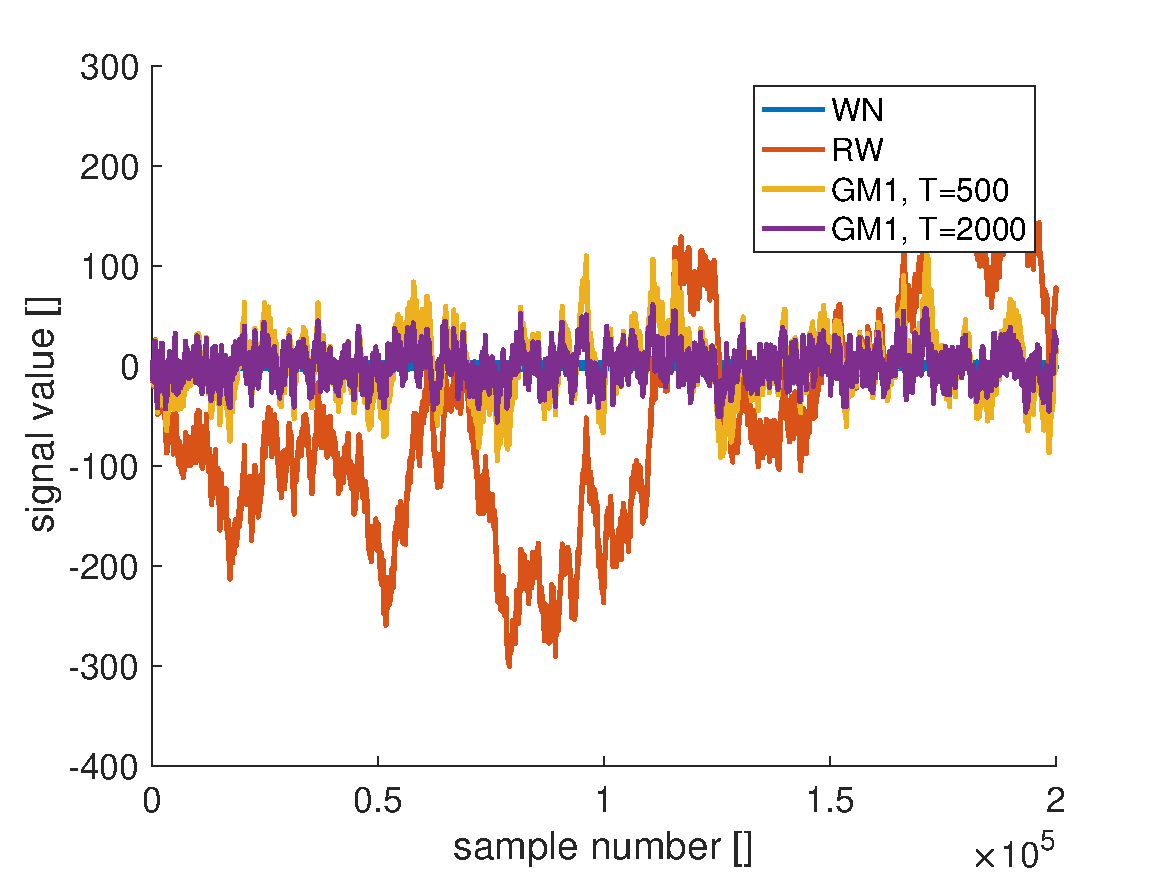
\includegraphics[width=\textwidth]{signal2}
\end{subfigure}
~
\begin{subfigure}[t]{0.49\textwidth}
\centering
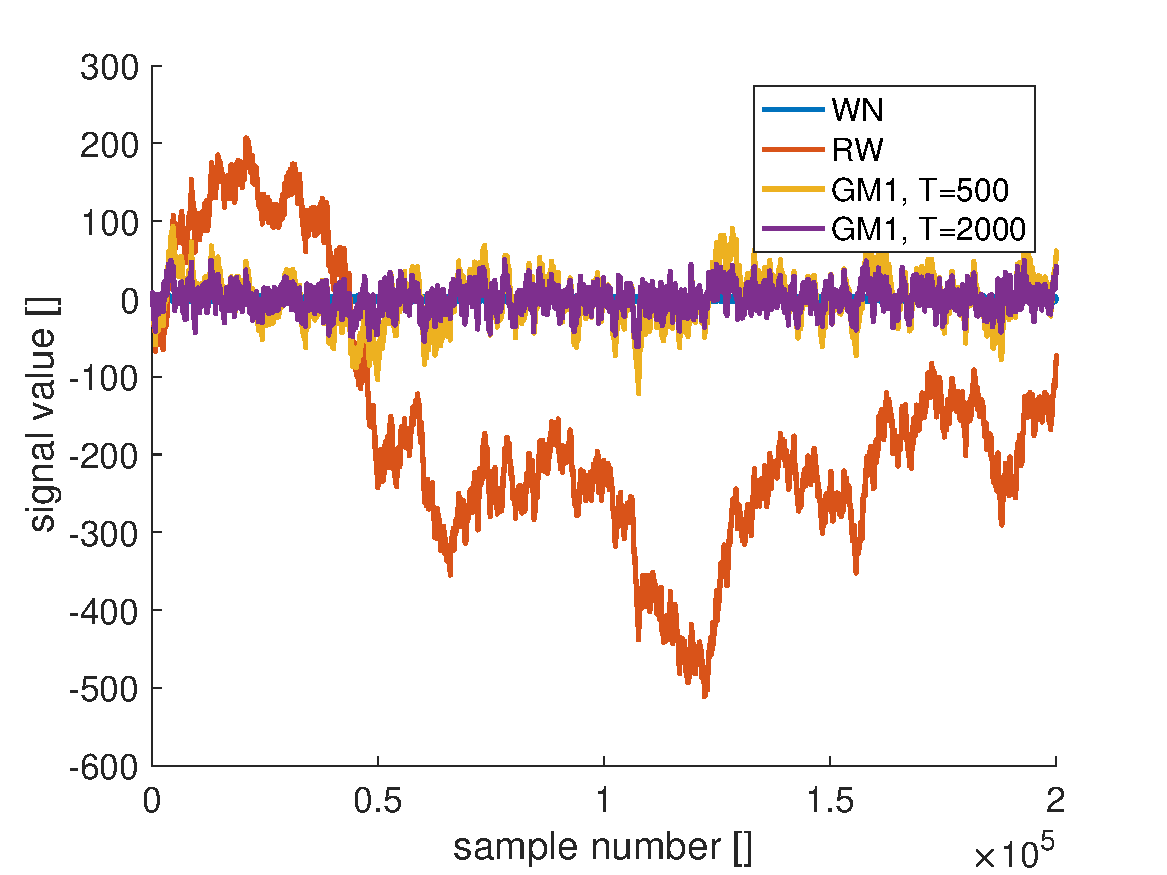
\includegraphics[width=\textwidth]{signal3}
\end{subfigure}
\caption{Three different realizations of White Noise (WN), Random Walk (RW) and first order Gauss-Markov (GM1) process with correlation times T=500 and T=2000.}
\label{fig:signals}
\end{figure}

\section*{2 }


\begin{figure}[H]
    \centering
    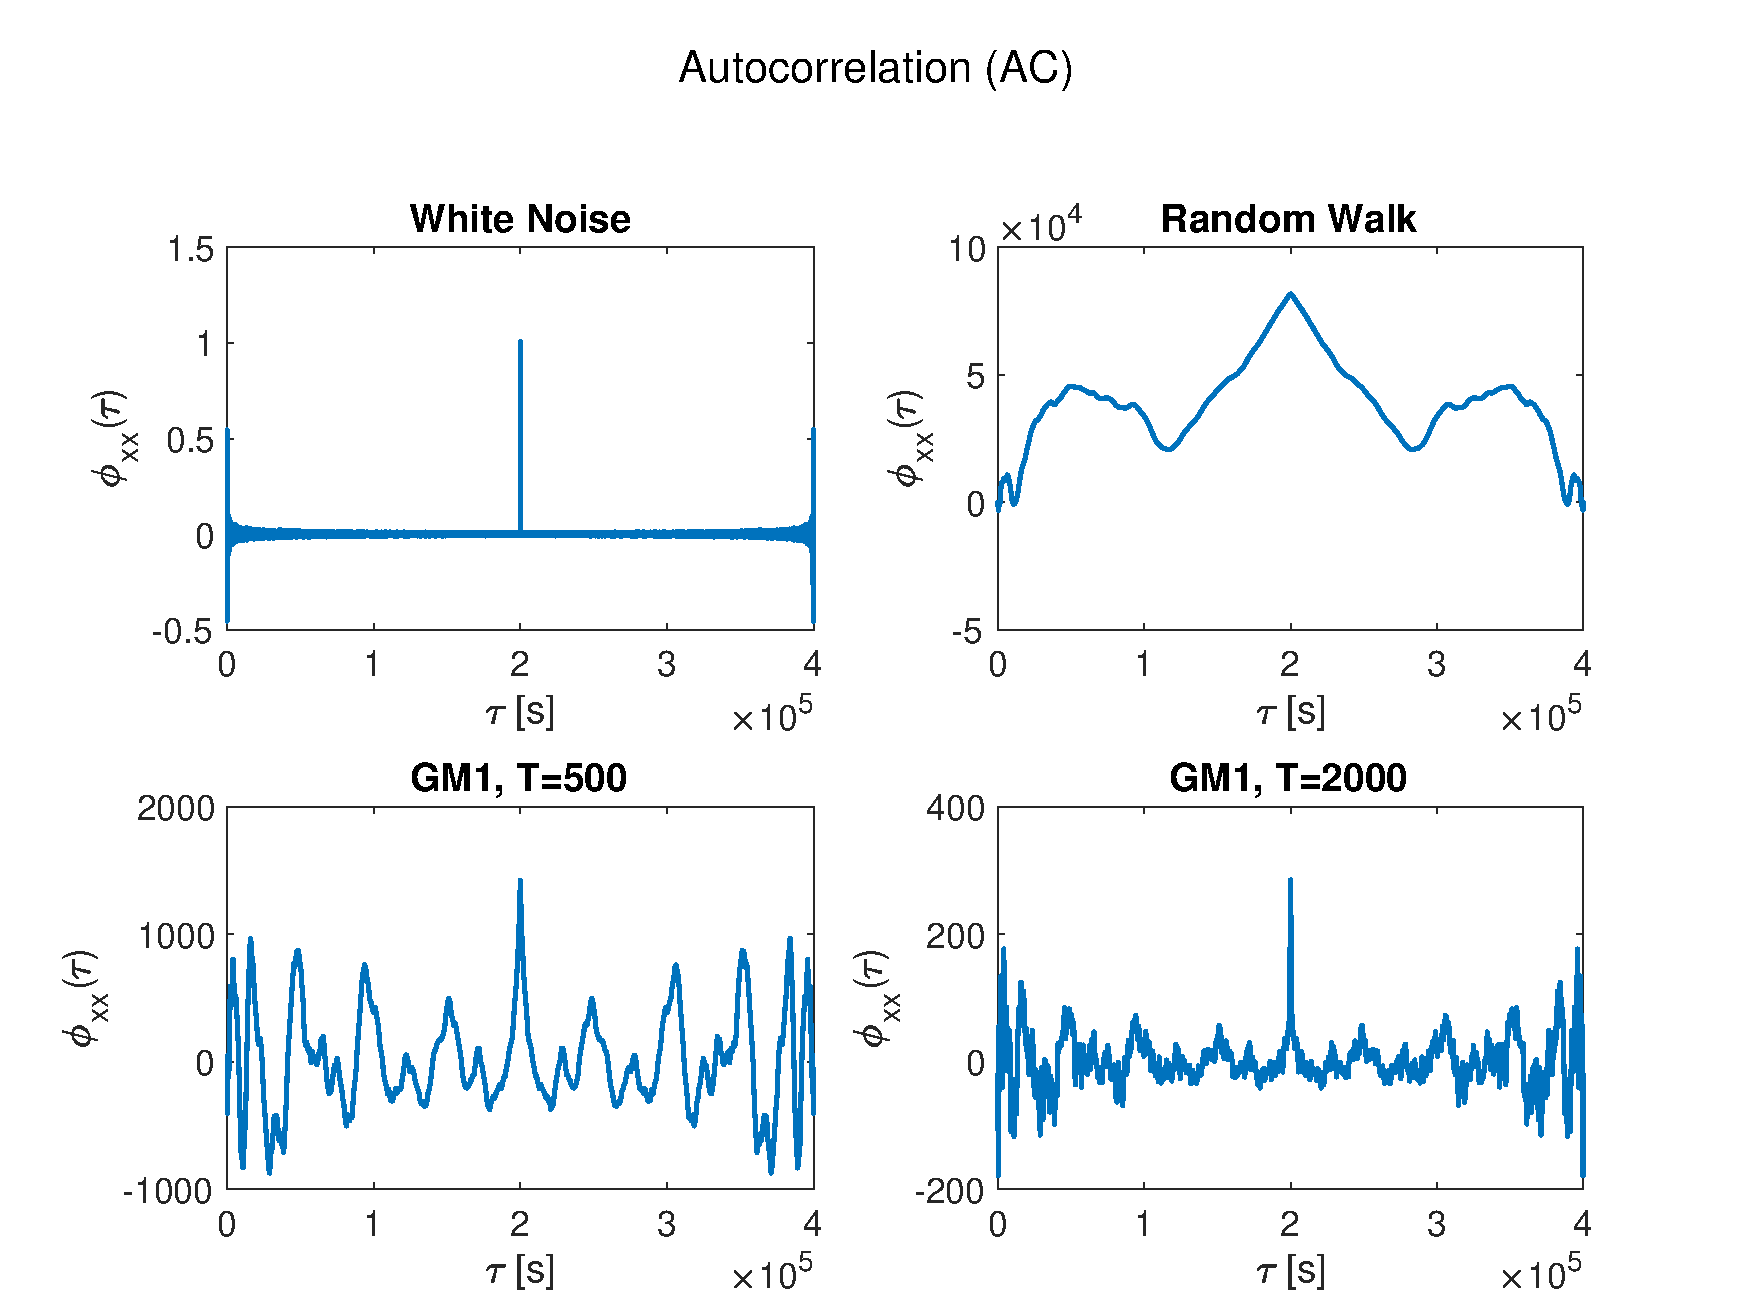
\includegraphics[width=\textwidth]{ac}
    \caption{Autocorrelation}
    \label{fig:autocorr}
\end{figure}

\begin{figure}[H]
    \centering
    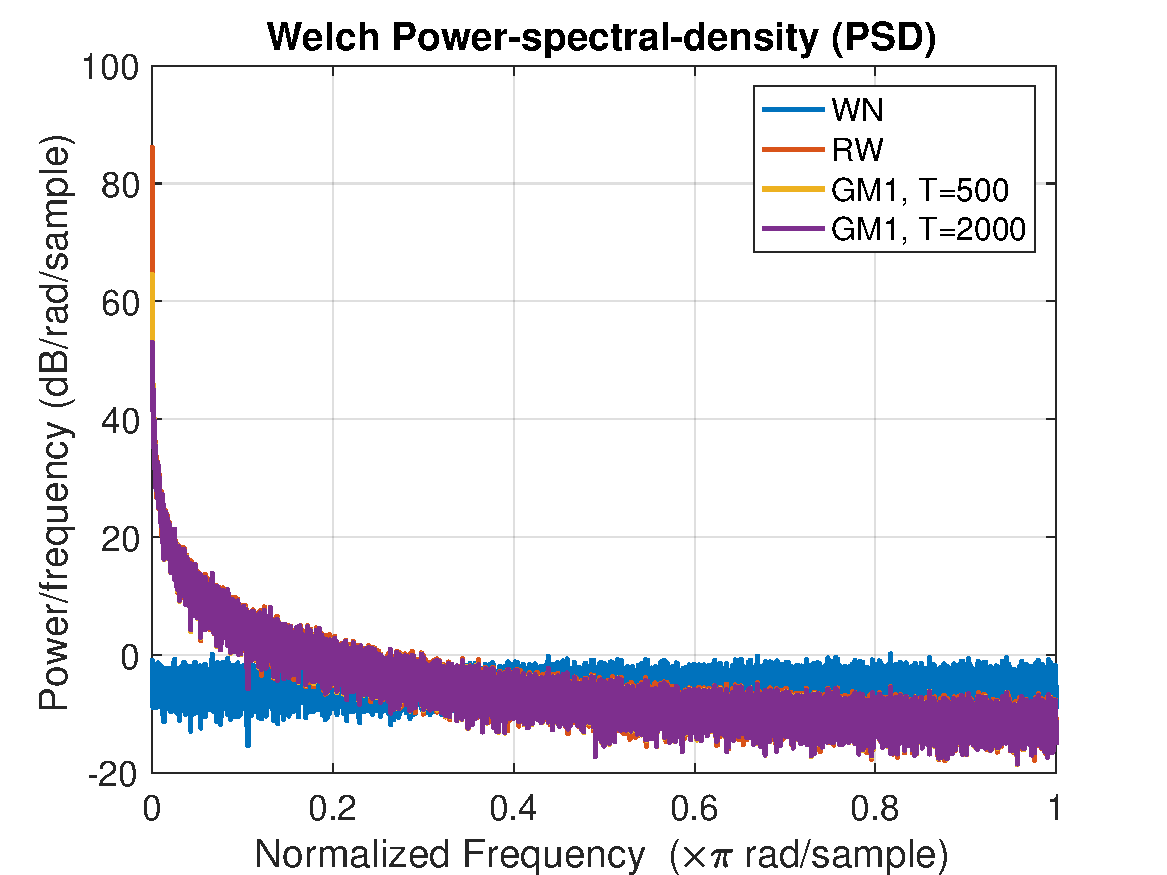
\includegraphics[width=0.5\textwidth]{psd}
    \caption{Power-spectral-density}
    \label{fig:autocorr}
\end{figure}

\newpage
\section*{Code}
\lstinputlisting{../lab1.m}


\end{document}
